\documentclass[17pt,a4paper,landscape]{extarticle}
\usepackage[margin=2.35cm,top=0.12cm,left=1.05cm]{geometry}
\usepackage{amsmath}
\usepackage{amssymb}
\usepackage{tasks}
\usepackage{tikz}
\usepackage{xcolor}
\usepackage[sfdefault,lf]{FiraSans}
\renewcommand{\familydefault}{\sfdefault}
\setlength{\parindent}{0pt}
\pagestyle{empty}
\settasks{label=\textbf{\arabic*.}, label-width=2.2em, item-indent=2.95em, column-sep=2.1cm, after-item-skip=9.8em}
\renewcommand{\arraystretch}{1.15}
\everymath{\displaystyle}

\begin{document}
\sffamily
\boldmath

\boldmath

\boldmath

{\LARGE \textbf{Drawing exponential graphs — Proficient}}\\[0.2em]
Use a sensible table of values. Mark the $y$-intercept before sketching the curve.

\begin{tasks}(4)
\task {Draw \mbox{$y=2^{x-1}$}. \\[0.4em] 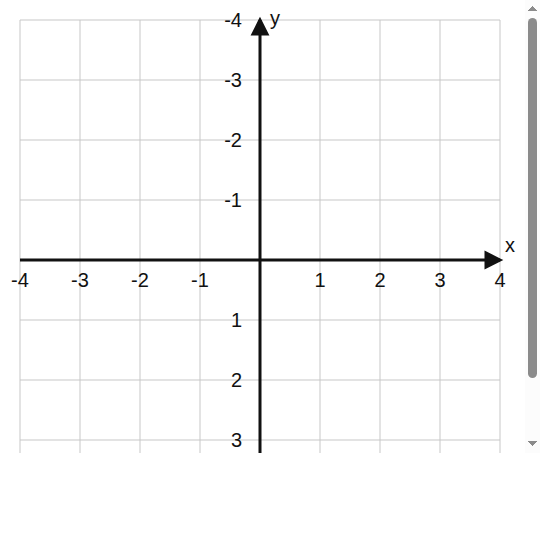
\includegraphics[width=0.88\linewidth]{web-diagrams/coord-grid.png}}
\task {Draw \mbox{$y=3^{x-1}$}. \\[0.4em] 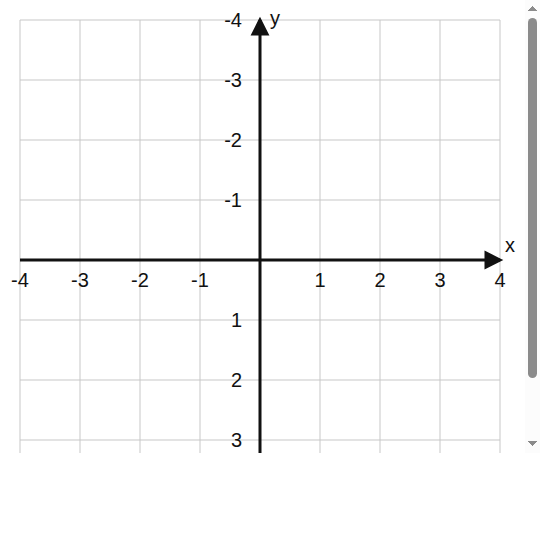
\includegraphics[width=0.88\linewidth]{web-diagrams/coord-grid.png}}
\task {Draw \mbox{$y=2^{x+2}$}. \\[0.4em] 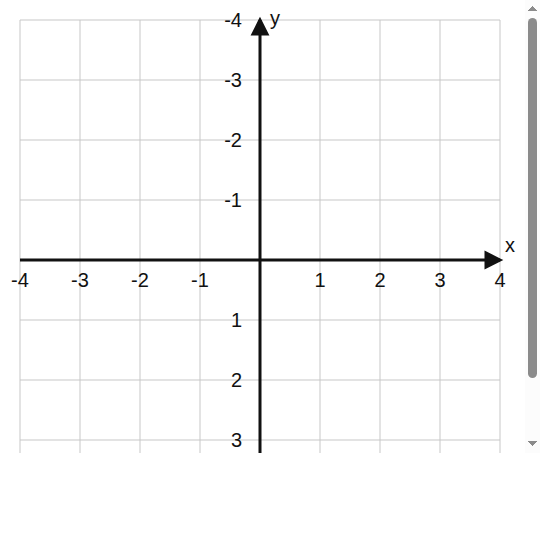
\includegraphics[width=0.88\linewidth]{web-diagrams/coord-grid.png}}
\task {Draw \mbox{$y=2^x+3$}. \\[0.4em] 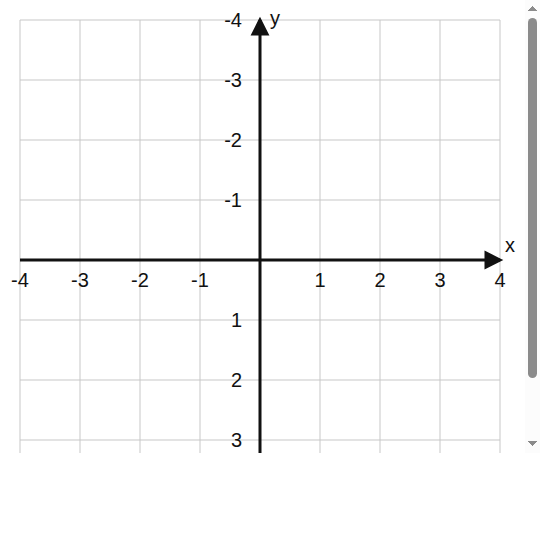
\includegraphics[width=0.88\linewidth]{web-diagrams/coord-grid.png}}
\task {Draw \mbox{$y=2^x-4$}. \\[0.4em] 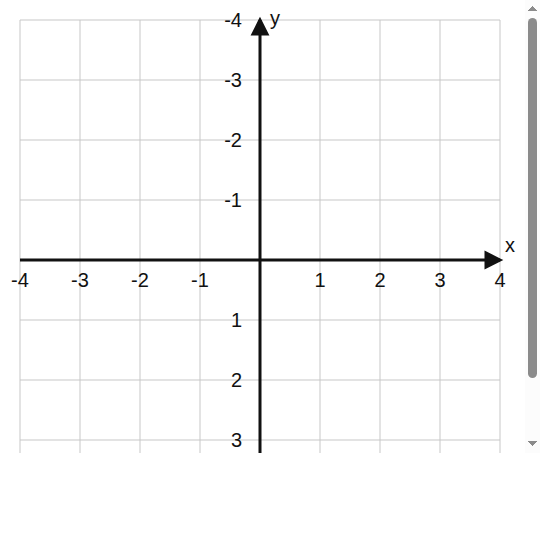
\includegraphics[width=0.88\linewidth]{web-diagrams/coord-grid.png}}
\task {Draw \mbox{$y=3\cdot 2^x+1$}. \\[0.4em] 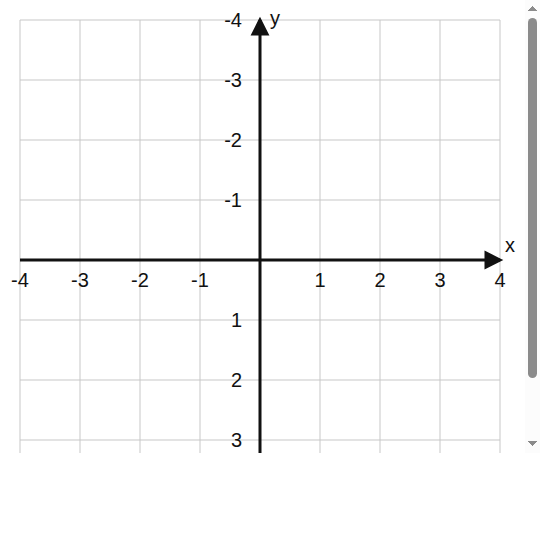
\includegraphics[width=0.88\linewidth]{web-diagrams/coord-grid.png}}
\task {Draw \mbox{$y=4\left(\frac{1}{2}\right)^x$}. \\[0.4em] 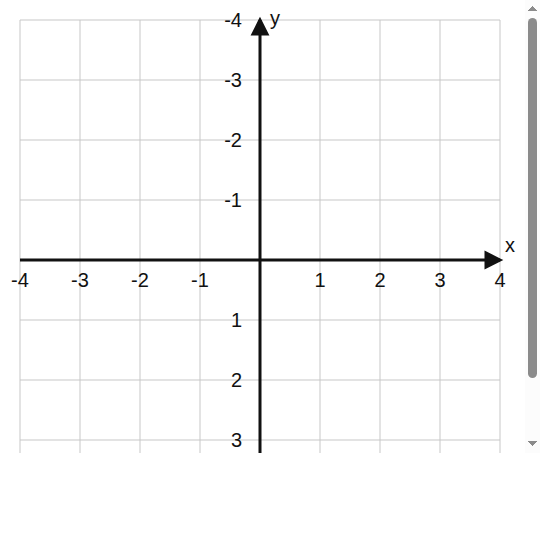
\includegraphics[width=0.88\linewidth]{web-diagrams/coord-grid.png}}
\task {Draw \mbox{$y=6\left(\frac{1}{3}\right)^x$}. \\[0.4em] 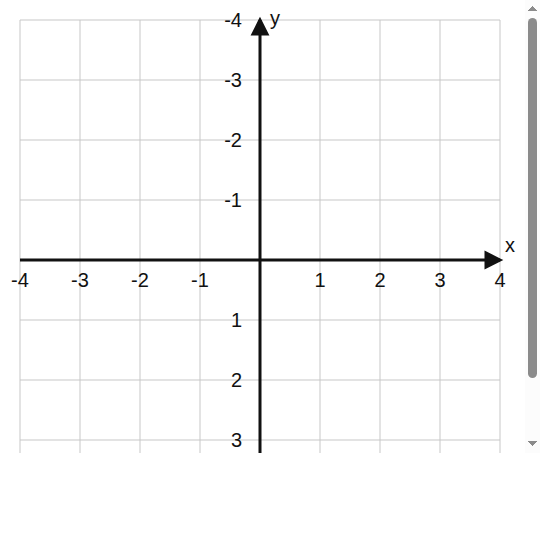
\includegraphics[width=0.88\linewidth]{web-diagrams/coord-grid.png}}
\task {Draw \mbox{$y=2\left(\frac{1}{2}\right)^x-1$}. \\[0.4em] 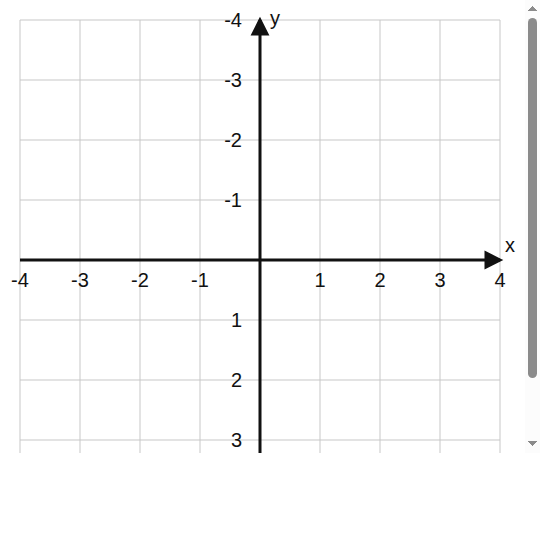
\includegraphics[width=0.88\linewidth]{web-diagrams/coord-grid.png}}
\task {Draw \mbox{$y=5\left(\frac{1}{2}\right)^x+2$}. \\[0.4em] 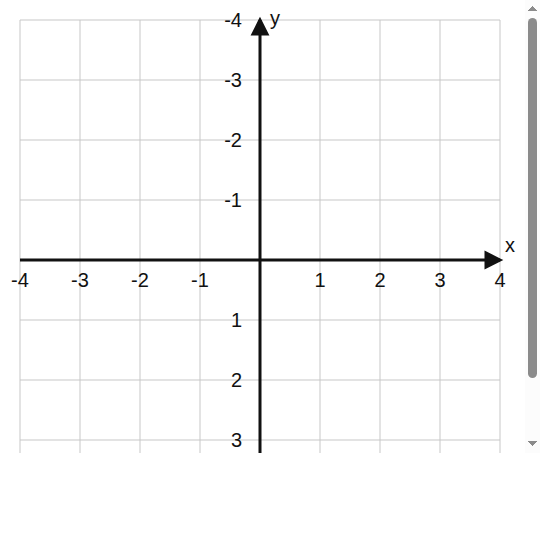
\includegraphics[width=0.88\linewidth]{web-diagrams/coord-grid.png}}
\task {Draw \mbox{$y=\frac{1}{4}\cdot 2^x$}. \\[0.4em] 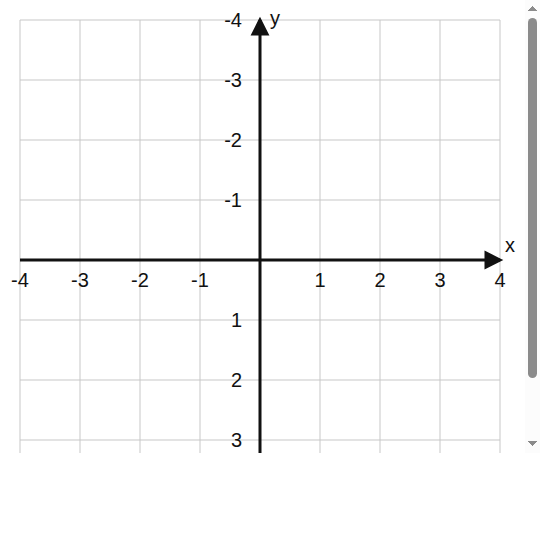
\includegraphics[width=0.88\linewidth]{web-diagrams/coord-grid.png}}
\task {Draw \mbox{$y=2\cdot 3^x-2$}. \\[0.4em] 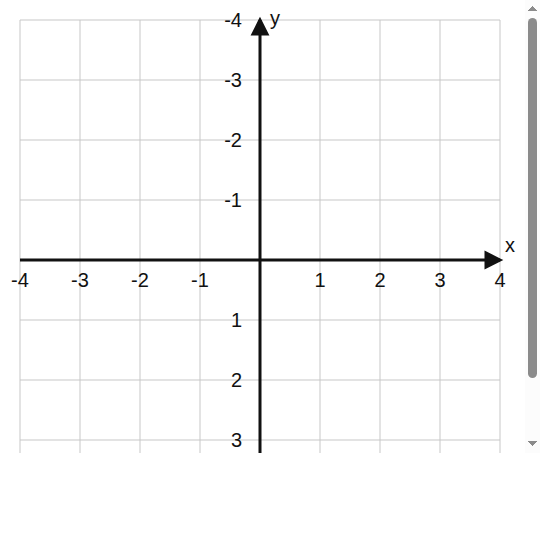
\includegraphics[width=0.88\linewidth]{web-diagrams/coord-grid.png}}
\end{tasks}

\end{document}
